\PassOptionsToPackage{dvipsnames,svgnames,x11names}{xcolor}
\documentclass[tikz,border=8pt]{standalone}
\usetikzlibrary{arrows.meta,positioning,calc,shapes,shadows,decorations.pathmorphing,shapes.geometric,backgrounds,decorations.markings,decorations.pathreplacing,decorations.text,fit,shapes.misc,shapes.arrows,matrix,bending,3d,chains,intersections,shapes.symbols,svg.path,shapes.multipart,snakes,shapes.callouts,angles,quotes}
\providecolor{gold}{RGB}{212,175,55}
\providecolor{silver}{RGB}{192,192,192}
\providecolor{bronze}{RGB}{205,127,50}
\providecolor{darkblue}{RGB}{0,0,139}
\providecolor{lightblue}{RGB}{173,216,230}
\providecolor{darkgreen}{RGB}{0,100,0}
\providecolor{lightgreen}{RGB}{144,238,144}
\providecolor{darkred}{RGB}{139,0,0}
\providecolor{navy}{RGB}{0,0,128}
\providecolor{skyblue}{RGB}{135,206,235}
\providecolor{beige}{RGB}{245,245,220}
\providecolor{cream}{RGB}{255,253,208}
\usepackage{amsmath}
\usepackage{amssymb}
\usepackage{fontawesome5}
\usetikzlibrary{fadings,shadows.blur,patterns,patterns.meta}


\providecolor{gold}{RGB}{212,175,55}
\providecolor{silver}{RGB}{192,192,192}
\providecolor{bronze}{RGB}{205,127,50}
\providecolor{darkblue}{RGB}{0,0,139}
\providecolor{lightblue}{RGB}{173,216,230}
\providecolor{darkgreen}{RGB}{0,100,0}
\providecolor{lightgreen}{RGB}{144,238,144}
\providecolor{darkred}{RGB}{139,0,0}
\providecolor{navy}{RGB}{0,0,128}
\providecolor{skyblue}{RGB}{135,206,235}
\providecolor{beige}{RGB}{245,245,220}
\providecolor{cream}{RGB}{255,253,208}

\usepackage{amsmath}
\usepackage{amssymb}
\usepackage{fontawesome5}

% --- DEFINED SEMANTIC COLORS ---
\definecolor{mathcolor}{RGB}{217, 119, 6}  % Deep Orange
\definecolor{funccolor}{RGB}{46, 125, 50}  % Forest Green
\definecolor{domcolor}{RGB}{2, 119, 189}   % Tech Blue
\definecolor{svgcolor}{RGB}{194, 24, 91}   % Crimson

\begin{document}
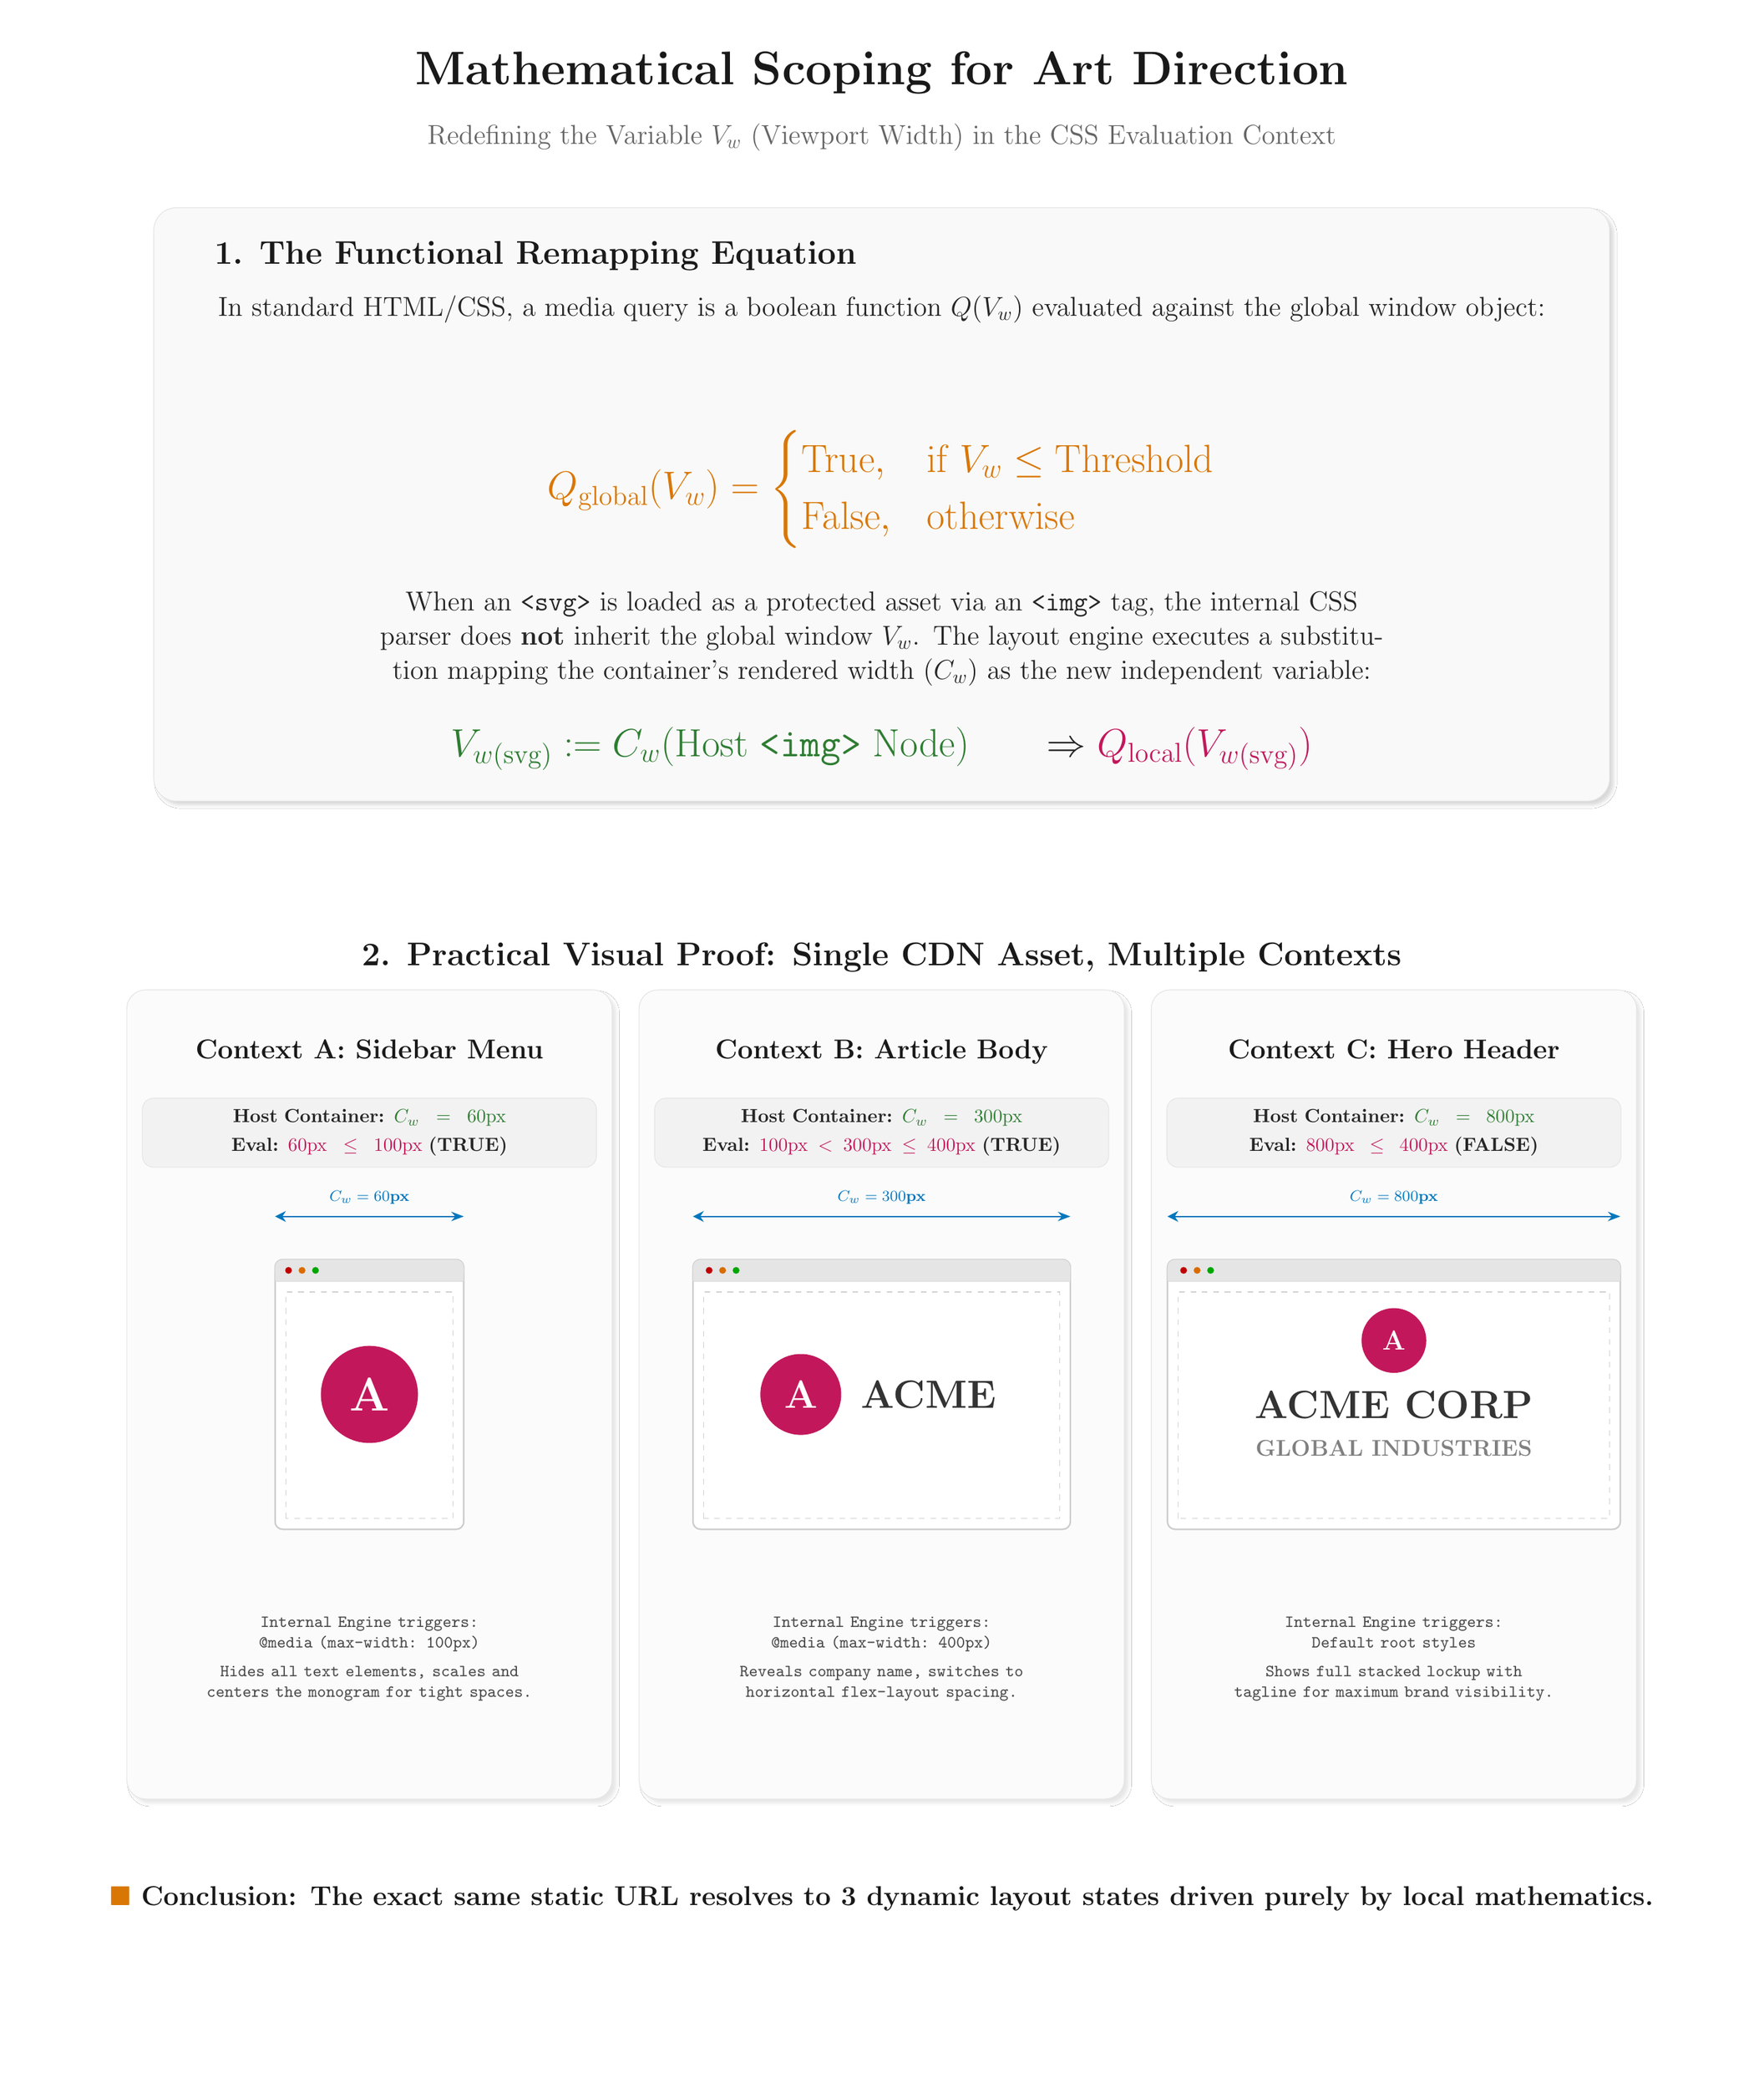
\begin{tikzpicture}[
    text=black!85,
    align=center
]

% =========================================================================
% 1. GLOBAL SETUP & CANVAS CONFIGURATION
% =========================================================================
\fill[white] (-16, -26) rectangle (16, 12);

% =========================================================================
% 2. TITLE & HEADER BLOCK
% =========================================================================
\node[font=\Huge\bfseries, text=black!90, anchor=center] at (0, 11.0) {Mathematical Scoping for Art Direction};
\node[font=\Large, text=black!60, anchor=center] at (0, 9.8) {Redefining the Variable $V_w$ (Viewport Width) in the CSS Evaluation Context};

% =========================================================================
% 3. SECTION 1: THE MATH THEORY
% =========================================================================
% Background Panel
\path[fill=gray!5, draw=gray!20, rounded corners=12pt, blur shadow={shadow opacity=15}] (-13.5, -2.5) rectangle (13.5, 8.5);

% Section Title
\node[font=\LARGE\bfseries, text=black!90, anchor=north west] at (-12.5, 8.0) {1. The Functional Remapping Equation};

% Paragraph 1
\node[font=\Large, text width=25cm, text=black!85, anchor=north] at (0, 7.0) {In standard HTML/CSS, a media query is a boolean function $Q(V_w)$ evaluated against the global window object:};

% Equation 1
\node[anchor=north] at (0, 4.5) {{\huge $\color{mathcolor} Q_{\text{global}}(V_w) = \begin{cases} \text{True}, & \text{if } V_w \le \text{Threshold} \\ \text{False}, & \text{otherwise} \end{cases}$}};

% Paragraph 2
\node[font=\Large, text width=25cm, text=black!85, anchor=north] at (0, 1.5) {When an \texttt{<svg>} is loaded as a protected asset via an \texttt{<img>} tag, the internal CSS parser does \textbf{not} inherit the global window $V_w$. The layout engine executes a substitution mapping the container's rendered width ($C_w$) as the new independent variable:};

% Equation 2
\node[anchor=north] at (0, -1.0) {{\huge $\color{funccolor} V_{w(\text{svg})} := C_w(\text{Host \texttt{<img>} Node})$ \hspace{1cm} $\Rightarrow \color{svgcolor} Q_{\text{local}}(V_{w(\text{svg})})$}};

% =========================================================================
% 4. SECTION 2: VISUAL PROOF & CONTEXT GRID
% =========================================================================
% Section Title
\node[font=\LARGE\bfseries, text=black!90, anchor=north] at (0.0, -5.0) {2. Practical Visual Proof: Single CDN Asset, Multiple Contexts};

% Context Cards (Backgrounds)
\path[fill=gray!3, draw=gray!20, rounded corners=10pt, blur shadow={shadow opacity=10}] (-14.0, -21.0) rectangle (-5.0, -6.0);
\path[fill=gray!3, draw=gray!20, rounded corners=10pt, blur shadow={shadow opacity=10}] (-4.5, -21.0) rectangle (4.5, -6.0);
\path[fill=gray!3, draw=gray!20, rounded corners=10pt, blur shadow={shadow opacity=10}] (5.0, -21.0) rectangle (14.0, -6.0);

% -------------------------------------------------------------------------
% COLUMN A LAYOUT (Center X: -9.5)
% -------------------------------------------------------------------------
\node[font=\Large\bfseries, text=black!90, anchor=north] at (-9.5, -6.8) {Context A: Sidebar Menu};

% Logic Box
\node[fill=gray!10, draw=gray!20, rounded corners=6pt, text width=8cm, inner sep=6pt, anchor=north] at (-9.5, -8.0) {
    \textbf{Host Container:} $\color{funccolor} C_w = 60\text{px}$\\[3pt]
    \textbf{Eval:} $\color{svgcolor} 60\text{px} \le 100\text{px}$ \textbf{(TRUE)}
};

% Dimension Line
\draw[{Stealth[length=2mm, width=2mm]}-Stealth=3mm, domcolor, thick] (-11.25, -10.2) -- (-7.75, -10.2);
\node[anchor=south, font=\footnotesize\bfseries, text=domcolor] at (-9.5, -10.1) {$C_w = 60\text{px}$};

% Browser Window Mockup
\filldraw[fill=white, draw=gray!40, thick, rounded corners=4pt] (-11.25, -16.0) rectangle (-7.75, -11.0);
\fill[gray!20, rounded corners=4pt] (-11.25, -11.4) rectangle (-7.75, -11.0);
\fill[gray!20] (-11.25, -11.4) rectangle (-7.75, -11.3);
\draw[gray!30] (-11.25, -11.4) -- (-7.75, -11.4);
% OS Window Controls
\fill[red!75!black] (-11.0, -11.2) circle (1.8pt);
\fill[orange!85!black] (-10.75, -11.2) circle (1.8pt);
\fill[green!65!black] (-10.5, -11.2) circle (1.8pt);
% Isolated CSS Context Boundary (Dashed)
\draw[dashed, gray!35] (-11.05, -15.8) rectangle (-7.95, -11.6);

% SVG Render: Monogram Only
\fill[svgcolor] (-9.5, -13.5) circle (0.9cm);
\node[text=white, font=\Huge\bfseries] at (-9.5, -13.5) {A};

% Trigger & Behavioral Description
\node[font=\small\ttfamily, text=black!70, text width=8cm, anchor=north] at (-9.5, -17.5) {
    Internal Engine triggers:\\
    \texttt{@media (max-width: 100px)}\\[4pt]
    Hides all text elements, scales and centers the monogram for tight spaces.
};

% -------------------------------------------------------------------------
% COLUMN B LAYOUT (Center X: 0.0)
% -------------------------------------------------------------------------
\node[font=\Large\bfseries, text=black!90, anchor=north] at (0.0, -6.8) {Context B: Article Body};

% Logic Box
\node[fill=gray!10, draw=gray!20, rounded corners=6pt, text width=8cm, inner sep=6pt, anchor=north] at (0.0, -8.0) {
    \textbf{Host Container:} $\color{funccolor} C_w = 300\text{px}$\\[3pt]
    \textbf{Eval:} $\color{svgcolor} 100\text{px} < 300\text{px} \le 400\text{px}$ \textbf{(TRUE)}
};

% Dimension Line
\draw[{Stealth[length=2mm, width=2mm]}-Stealth=3mm, domcolor, thick] (-3.5, -10.2) -- (3.5, -10.2);
\node[anchor=south, font=\footnotesize\bfseries, text=domcolor] at (0.0, -10.1) {$C_w = 300\text{px}$};

% Browser Window Mockup
\filldraw[fill=white, draw=gray!40, thick, rounded corners=4pt] (-3.5, -16.0) rectangle (3.5, -11.0);
\fill[gray!20, rounded corners=4pt] (-3.5, -11.4) rectangle (3.5, -11.0);
\fill[gray!20] (-3.5, -11.4) rectangle (3.5, -11.3);
\draw[gray!30] (-3.5, -11.4) -- (3.5, -11.4);
% OS Window Controls
\fill[red!75!black] (-3.2, -11.2) circle (1.8pt);
\fill[orange!85!black] (-2.95, -11.2) circle (1.8pt);
\fill[green!65!black] (-2.7, -11.2) circle (1.8pt);
% Isolated CSS Context Boundary (Dashed)
\draw[dashed, gray!35] (-3.3, -15.8) rectangle (3.3, -11.6);

% SVG Render: Monogram + ACME Flex
\fill[svgcolor] (-1.5, -13.5) circle (0.75cm);
\node[text=white, font=\huge\bfseries] at (-1.5, -13.5) {A};
\node[font=\huge\bfseries, text=black!80, anchor=west] at (-0.5, -13.5) {ACME};

% Trigger & Behavioral Description
\node[font=\small\ttfamily, text=black!70, text width=8cm, anchor=north] at (0.0, -17.5) {
    Internal Engine triggers:\\
    \texttt{@media (max-width: 400px)}\\[4pt]
    Reveals company name, switches to horizontal flex-layout spacing.
};

% -------------------------------------------------------------------------
% COLUMN C LAYOUT (Center X: 9.5)
% -------------------------------------------------------------------------
\node[font=\Large\bfseries, text=black!90, anchor=north] at (9.5, -6.8) {Context C: Hero Header};

% Logic Box
\node[fill=gray!10, draw=gray!20, rounded corners=6pt, text width=8cm, inner sep=6pt, anchor=north] at (9.5, -8.0) {
    \textbf{Host Container:} $\color{funccolor} C_w = 800\text{px}$\\[3pt]
    \textbf{Eval:} $\color{svgcolor} 800\text{px} \le 400\text{px}$ \textbf{(FALSE)}
};

% Dimension Line
\draw[{Stealth[length=2mm, width=2mm]}-Stealth=3mm, domcolor, thick] (5.3, -10.2) -- (13.7, -10.2);
\node[anchor=south, font=\footnotesize\bfseries, text=domcolor] at (9.5, -10.1) {$C_w = 800\text{px}$};

% Browser Window Mockup
\filldraw[fill=white, draw=gray!40, thick, rounded corners=4pt] (5.3, -16.0) rectangle (13.7, -11.0);
\fill[gray!20, rounded corners=4pt] (5.3, -11.4) rectangle (13.7, -11.0);
\fill[gray!20] (5.3, -11.4) rectangle (13.7, -11.3);
\draw[gray!30] (5.3, -11.4) -- (13.7, -11.4);
% OS Window Controls
\fill[red!75!black] (5.6, -11.2) circle (1.8pt);
\fill[orange!85!black] (5.85, -11.2) circle (1.8pt);
\fill[green!65!black] (6.1, -11.2) circle (1.8pt);
% Isolated CSS Context Boundary (Dashed)
\draw[dashed, gray!35] (5.5, -15.8) rectangle (13.5, -11.6);

% SVG Render: Full Stacked Lockup
\fill[svgcolor] (9.5, -12.5) circle (0.6cm);
\node[text=white, font=\Large\bfseries] at (9.5, -12.5) {A};
\node[font=\huge\bfseries, text=black!80, anchor=center] at (9.5, -13.7) {ACME CORP};
\node[font=\large\bfseries, text=gray, anchor=center] at (9.5, -14.5) {GLOBAL INDUSTRIES};

% Trigger & Behavioral Description
\node[font=\small\ttfamily, text=black!70, text width=8cm, anchor=north] at (9.5, -17.5) {
    Internal Engine triggers:\\
    \texttt{Default root styles}\\[4pt]
    Shows full stacked lockup with tagline for maximum brand visibility.
};

% =========================================================================
% 5. CONCLUSION BLOCK
% =========================================================================
\node[font=\Large\bfseries, text=black!90, anchor=north] at (0, -22.5) {$\color{mathcolor}\blacksquare$ Conclusion: The exact same static URL resolves to 3 dynamic layout states driven purely by local mathematics.};

\end{tikzpicture}
\end{document}
